\chapter{Superficies compactas}

\section{Superfies topológicas}

En primer lugar recordaremos algunos conceptos de Topología I para poder definir los nuevos conceptos de esta sección.

\begin{definicion}
    Diremos que un espacio topológico $X$ es T2 (o de \textbf{Haussforff}, o que satisface el \textbf{segundo axioma de separación}) si $\forall x,y \in X$ existe un abierto $U$ que contenga a $x$ y un abierto $V$ que contenga a $y$ tal que $U\cap V = \emptyset$.
        
        \begin{center}
            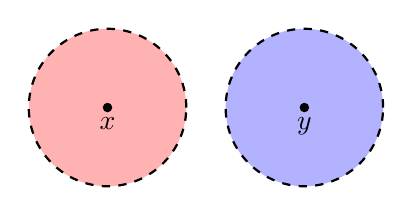
\begin{tikzpicture}
                \centering
    
                \def\radius{1}
    
                % Desactiva los caracteres conflictivos
                \shorthandoff{>} % Para poner puntas de flecha
    
                % Background
                \fill[fill=red!30] (-1,0) circle (\radius);
                \fill[fill=blue!30] (1.5,0) circle (\radius);
    
                \draw[dashed, thick] (-1,0) circle (\radius);
                \filldraw (-1,0) circle (1.5pt)  node[below] {$x$};
                \draw[dashed, thick] (1.5,0) circle (\radius);
                \filldraw (1.5,0) circle (1.5pt)  node[below] {$y$};
    
            \end{tikzpicture}
        \end{center}
\end{definicion}

\begin{definicion}
    Decimos que un espacio topológico $X$ es 2AN (o que cumple el \textbf{segundo axioma de numerabilidad}) si existe una base de la topología numerable.
\end{definicion}

\begin{definicion}
    Decimos que un espacio topológico $X$ es \textbf{localmente euclídeo} si para coda $x\in X$ existe un entorno abierto suyo que es homeomorfo a un abierto de $\bb{R}^n$.\\

    Decimos que $S$ es una \textbf{superficie} si $S$ es un espacio topológico tal que $\forall x \in S$ existe un abierto que contiene a $x$ y que es homeomorfo a un abierto de $\bb{R}^2$. Además, pediremos que $S$ sea T2 (o Hausdorff) y 2AN (segundo axioma de numerabilidad).
\end{definicion}

\begin{ejemplo}\
    \begin{enumerate}
        \item $\bb{R}^2$ y $\bb{S}^2$ son superficies.
        \item Cualquier abierto de una superficie es también una superficie. En particular, las bolas abiertas de $\bb{R}^2$ son también superficies.
        \item Sea $X=\{x\in \bb{R}^2 : \|x\|\leq r\} = \overline{B}(0,r)$. Entonces $X$ no es una superficie porque para los puntos $x$ con $\|x\| = r$ no existe un entorno abierto que lo contenga y que sea homeomorfo a un abierto de $\bb{R}^2$.
        \begin{proof}
            Tomamos un punto $x\in X$ con $\|x\|=r$. Si existiese $U$ entorno abierto suyo homeomorfo a un abierto $A$ de $\bb{R}^2$ entonces $\exists V$ entorno abierto de $x$ contenido en $U$ que es de la forma $V=B(x,r_0)\cap X$. Entonces $V$ es homeomorfo a un abierto $A'$ de $\bb{R}^2$ (ya que sería una restricción en el dominio del homeomorfismo entre $h:U\to A$). De esta forma tendríamos que como $V\setminus \{x\}$ es convexo debe ser simplemente conexo. Sin embargo, su imagen por homeomorfismo $h$ será $A'\setminus \{h(x)\}$ y como $h(x)$ está en el abierto $A'$ existe un radio $r_0'>0$ tal que $\overline{B}(h(x),r_0') \subseteq A'$. Pero el lazo dado por la frontera de dicha bola, $Fr(\overline{B}(h(x)r_0'))$ no es homotópicamente constante en $\bb{R}^2\setminus \{h(x)\}$. Por tanto este lazo no es homotópicamente constante en $A'\setminus\{h(x)\}$ por lo que $A'\setminus\{h(x)\}$ no es simplemente conexo. Esto prueba que $\overline{B}(0,r)$ no es una superficie.
        \end{proof}

        \item $\bb{S}^1\times \bb{R}$ y $\bb{S}^1\times \bb{S}^1$ son ejemplos de superficies. Esto se debe a que su recubridor universal es $\bb{R}^2$ luego sus aplicaciones recubridoras nos dan homeomorfismos locales desde abiertos de $\bb{R}^2$ en abiertos regularmente recubiertos de $\bb{S}^1 \times \bb{R}$ o $\bb{S}^1\times \bb{S}^1$.
    \end{enumerate}
\end{ejemplo}

\begin{observacion}
    Si $X$ es un espacio topológico localmente euclídeo entonces cumple las propiedades locales de $\bb{R}^n$. Por ejemplo, tiene una base de entornos numerable (es 1AN) y es localmente simplemente conexo. En particular, $X$ ha de tener recubridor universal.
\end{observacion}

\begin{definicion}
    Sea $S$ una superficie\footnote{siempre se entiende que es una superficie topológica} y $D$ un abierto dentro de $S$. Decimos que $D$ es un \textbf{disco regular} en $S$ si existe un aberto $D'$ tal que $D\subsetneq D'$ y un homeomorfismo $h:D'\to \bb{D}=\{x\in \bb{R}^2 : \|x\|<1\}=B(0,1)$ tal que $h(D)=\bb{D}_r=\{x\in \bb{R}^2 : \|x\|<r\}=B(0,r)$ con $0<r<1$.
\end{definicion}

\begin{ejemplo}\
    \begin{enumerate}
        \item Consideramos en $\bb{S}^2$:
        \begin{gather*}
            D = \{(x,y,z)\in \bb{S}^2 : z<r\} \text{ con } -1<r<1
        \end{gather*}
        En efecto es un disco regular.

        \item Consideramos 
    \end{enumerate}
\end{ejemplo}